%\documentclass[prb,preprint]{revtex4} 
\documentclass[twocolumn,preprintnumbers,amsmath,amssymb,aps,prx]{revtex4}
% The line above defines the type of LaTeX document.
% Note that AJP uses the same style as Phys. Rev. B (prb).

% The % character begins a comment, which continues to the end of the line.
\usepackage{amsmath}  % needed for \tfrac, \bmatrix, etc.
\usepackage{amsfonts} % needed for bold Greek, Fraktur, and blackboard bold
\usepackage{graphicx} % needed for figures
\usepackage{pythontex}

\begin{document}

% Be sure to use the \title, \author, \affiliation, and \abstract macros
% to format your title page.  Don't use lower-level macros to  manually
% adjust the fonts and centering.

\title{Molecular dynamics simulation of synchronization in driven particles}
% In a long title you can use \\ to force a line break at a certain location.

\author{Tiare Guerrero}
\email{guer9330@pacificu.edu} % optional
%\altaffiliation[permanent address: ]{101 Main Street, 
%  Anytown, USA} % optional second address
% If there were a second author at the same address, we would put another 
% \author{} statement here.  Don't combine multiple authors in a single
% \author statement.
\affiliation{Department of Physics, Pacific University, Forest Grove, OR 97116}
% Please provide a full mailing address here.

\author{Danielle McDermott}
\email{mcdermott@pacific.edu}
\affiliation{Department of Physics, Pacific University, Forest Grove, OR 97116}

% See the REVTeX documentation for more examples of author and affiliation lists.
\date{\today}

\begin{abstract}
  %What problem did you study and why is it important?
  We discuss a
  numerical model
  of particles
  confined to a narrow channel 
  driven
  across a washboard potential energy landscape.
  The model 
  exhibits
  synchronization effects that provide insight
  to the behavior of 
  many experimental systems of
  interest to condensed matter physics 
  including 
  magnetically driven colloidal particles
  confined by light-fields, 
  voltage driven superconducting vortices
  confined in a Josephson junction,
  and ac and dc driven
  charge and spin density waves.
  We present the basics
  of the molecular dynamics simulations
  for particles moving through
  a viscous liquid.
  %so we model the dynamics of each particle
  %with 
  %overdamped equations of motion.
  We demonstrate how to visualize
  the system
  and measure hallmarks of synchronization, 
  Shapiro steps,
  that exhibit non-Ohmic step-like behavior 
  in the 
  the particle velocity as a function of applied driving force.
  We include sample code
  and exercises for students
  %that include
  with 
  opportunties
  to reproduce our results and propose
  new numerical experiments.
  With only a few particles in two-dimensions,
  the simulation runs quickly,
  making this an appropriate model for undergraduates to explore.

  %Hew to this recipe (MMRC) witlessly
  %1. M—Give the motivation and context
  %2. M—Explain what you did in sufficient
  %detail so the audience knows if your work
  %is relevant and applicable to his or hers
  %3. R—Emphasize your key results
  %4. C—Tell the reader what you think the
  %results mean
  
\end{abstract}
% AJP requires an abstract for all regular article submissions.
% Abstracts are optional for submissions to the "Notes and Discussions" section.

\maketitle % title page is now complete

\section{Introduction} %
%
%Outline
%------------------------------------------------------------------
%synchronization = widest audience possible
Synchronization is a universal phenomena
in which individual oscillators adjust rhythm due
to an external stimuli \cite{Pikovsky2003}.
%Christiaan Huygens 
%[has been adapted into many useful technologies...]
Synchronization was first reported in the scientific literature
when in 1665 
Huygens' experiments on
the 
motions of two pendula on wall-mounted clocks 
demonstrated the tendency of 
two periodic oscillators in close
proximity to swing in time, i.e. to synchronize,
due to interactions through the wall \cite{Bennett2002}.
Synchronous behaviors are observed
in many everyday systems
such as the
flickering candle flames coupled by temperature fluctuations \cite{Okamoto2016} 
and metronomes coupled through the the supporting table \cite{Jia2015}.
Biological systems benefit from cooperative
synchronzation such as when 
birds coordinate
flapping of wings in order to optimize energy use during flight \cite{Portugal2014},
frogs communicate by croaking patterns dictated by location \cite{Aihara2014},
and humans synchronize clapping in time with music \cite{Tranchant2016}.
At a cellular level, 
neurons simultaneously fire in cardiac muscle \cite{MartinHall1999}
and brain tissue \cite{Singer1999}.

Synchronization is also referred to as 
phase-locking or mode-locking.
%phase locking
Dynamical systems %with multiple frequencies
exhibit phase-locking 
when oscillators with different frequencies couple
so the frequency ratio or mode 
is an integer number \cite{Bak1986} .
This can be demonstrated
with Lissajous figures, i.e. parametric graphs of two periodic functions
which make looped patterns determined by the mode, % frequency ratio,
first reported in 1857 \cite{Lissajous1857}
and easily generated with a computer code 
or oscilloscope \cite{Tong1997}. 
%with a frequency generator,
%where two combined frequencies at perpendicular orientations 

Synchronization is often achieved via external forcing.
Examples of synchronization via external forcing include
pushing a child on a swing or
using a pacemaker (an electrical generator)
that pulses to regulate a heart beat.
This kind of 
dynamical mode locking
is often observed in quantum electronic
devices such as Josephson junctions \cite{Josephson1962,Josephson1965}
i.e. phase-locked current loops \cite{} 
which exhibit phase locking via
stepped regions in current-voltage (I-V) 
instead of ohmic relationships.
Also known as Shapiro steps \cite{Shapiro1963},
these steps have been observed broadly in 
velocity-force curves and voltage-current curves
as indicators of phase locking \cite{Golubov2004}.

Recent work with atomic systems such as Bose-Einstein condensates \cite{Zhang2020}

Synchronization has many important
technological applications
and is often studied with simplified computational models.
%mini review of synchronization in electronics
%careful - the following is all simulations
Recent studies demonstrate
that coupled electronic oscillators can be
programmed for use as microcontrollers for robotic locomotion \cite{Dutta2019}.

%Given the prevalence of synchronization,
%it is the subject of many computational models.
Here we focus numerical studies 
of the synchronized dynamics
of confined particles driven over
a washboard shaped potential energy landscape. 
We chose this model for its
relevance to condensed matter systems



Studies modeling synchronized behaviors
can be performed with
coupled oscillators []
An alternative method is to
study the dynamics of a single particle
confined in a periodic 
potential landscape subject
to with an applied driving force with constant or direct (DC)
and alterating (AC)
components.

Relationship between substrate period and intrinsic velocity
with phase locking caused by AC force modulates drive
where the particle velocity is constant even though the applied
DC force is increased.



Recent experiments of particles confined
in optical traps
subject to external driving forces 
have
been used to examine the microscopic dynamics
of mode-locking in colloids \cite{juniper2015} and ions \cite{Bushev2013}.
%experimental - colloids specifically
Colloidal particles trapped in light fields are %have proven
a particularly useful medium for studying complex dynamical behaviors.  %cite 
The relatively large size of the colloids (micrometers)
makes colloids easy to control and image,
and the interaction forces between colloids can be modified
by tuning the chemistry of the suspending fluid or surface ligands
of the colloidal particles \cite{Grier2003}.
This ease in control of colloids has lead to a rich array of 
experimental results  
considered models
for experimental systems relatively hard to access and visualize,
such as cold atoms or electron gases. %ELABORATE AND CITE

%-----------------------------------------------------------
%particle interaction types
Particles which interact over long distances
include colloids, magnetic beads, superconducting vortices, dusty plasmas, electron gases. [more detail and references]
Particles which interact over short distances include
bubble arrays/emulsions [more systems and references].

%-----------------------------------------------
%environments
Particles in confined geometries behave differently than free particles.
Stabilized charged particles form patterns
due to the interplay of the confining environment
and particle interactions.
Narrow channels studies are useful to provide insights 
of how particles move through systems 
such as wires and microchannels.
Biological systems such as
neuron axons and capillaries can also be studied
with these models [more detail and references].
Many such systems execute local oscillations
about stable points [elaborate].
%----------------------------------------------------------
The presence of a modulating surface
can modify these patterns in a variety of ways,
changing the onset of dynamical flows,
and the overall flow patterns.
%

%external forces
The
dynamics of particles subject to 
an applied external force apply to many physical systems.
For instance the flow of charges in a conductor,
or cells responding to a chemical gradient.
The external force 
increases the diversity of dynamical behaviors,
and can cause particles to flow in
a variety of non-linear complex patterns
that may be 
synchronized.
Disordered chaotic dynamics are also possible,
where irregular, unpredictable time evolution of
nonlinear systems and occurs in mechanical oscillators \cite{chaos}.

%-------------------------------------------------------------

Numerical modeling of colloids can provide mechanistic insight
that can be difficult to achieve in experimental conditions
where Brownian motion and other sources of noise dominate.
[elaborate]

%another confinement technique:
%Acoustic tweezers and surface acoustic wave (SAW) \cite{}
%confines single cells and particles with lower energy than light / lasers
%%X. Ding, J. Shi, S.-C. S. Lin, S. Yazdi, B. Kiraly and T. J. Huang, “Tunable patterning of microparticles and cells using standing surface acoustic waves” Lab Chip, 2012, 12, 2491– 2497.
%%%Acousto-optically generated potential energy landscapes: Potential mapping using colloids under flow Michael P. N. Juniper,1,∗ Rut Besseling,2 Dirk G. A. L. Aarts,1 and Roel P. A. Dullens1

%---------------------------------------------------------------
%kinks and nanofriction

%-----------------------------------------------------------------
%transition from synchronized to chaotic

%describe types of physical systems - particle types
In this work,
we perform 
numerical simulations of confined, driven particles
to model a variety of physical phenomena.
%----------------------------------------------------------------------------
%paper outline
In the following paper we describe
our molecular dynamics model in Section~\ref{sec:MD}.
%including various  and confining environments.
We include code to simulate
and visualize the dynamics in this section
and supplementary material.
In Section~\ref{sec:results} we summarize
our results,
including synchronized motion of a single confined particle
driven across a periodic landscape in 
Section~\ref{sec:one} and
multiple interacting particles
in Section~\ref{sec:sync},
including stationary propagation of high density kinks
in Sec.~\ref{sec:kink}.
%we
%demonstrate how uniform environments and applied forces
%and create synchronized flow patterns.
We present these results using standard tools of non-linear oscillators
such phase diagrams of velocity versus position.
In Section~\ref{sec:quasiperiod},
we show how an aperiodic landscape modifies the particle dynamics.
Finally we explore the transition to chaotic dynamics in 
Section~\ref{sec:chaos}
and conclude 
in Section~\ref{sec:conclusion}. 
In each section
we suggest exercises for interested students,
as summarized in Section~\ref{sec:problems}.


%Here we model the microscopic dynamics of phase locking in a colloidal model system using molecular dynamics (MD).

\section{Molecular Dynamics Model}
\label{sec:MD}
We use a classical two-dimensional model for 
studying the dynamics of $N$ interacting particles. 
Particles are confined in a two-dimensional (2D) 
simulation of area $A = L \times L$ where $L=36.5 a_0$
where $a_0$ is a dimensionless unit of length.
An individual particle $i$ has
position $\vec{r}_i = x_i \hat{x} + y_i \hat{y}$.
Particles are subject to
periodic boundary conditions
such that a particle leaving the edges of the system is mapped
back to a position within the simulation 
by $x_i+L=x_i$ and $y_i+L=y_i$.
The units of the simulated variables are in Table ~\ref{tab:1}.

\begin{table}[h!]
\centering
\caption{Simulation units.}
\begin{ruledtabular}
\begin{tabular}{c c p{5cm}}
Quantity & Unit \\
\hline
length &  $a_0$ \\
%electric potential & $V(r_{ij}) = E_0/r_{ij}$ \\
energy & $E_0 = q^2{Z^*}^2/4\pi \epsilon \epsilon_0 a_0$ \\
dimensionless interaction strength & $q$ \\
effective colloidal charge & $Z^*$ \\
solvent dielectic constant & $\epsilon \epsilon_0$\\
force & $E_0 / a_0$\\
viscosity/damping constant & $\eta$ \\
time &  $\eta / E_0$ \\
velocity &  $ E_0 / \eta a_0$ \\
\end{tabular}
\end{ruledtabular}
\label{tab:1}
\end{table}

We model particle interaction forces
$\vec{F}_{ij} = -\nabla U_{ij}(r_{ij})$ 
with
the Yukawa potential energy 
\begin{equation}
  U_{ij}(r_{ij}) = \frac{E_0}{r_{ij}} e^{-\kappa r_{ij}},
\end{equation}
where particle $i$ and $j$ are distance
$r_{ij} = |\vec{r}_i - \vec{r}_j|$ apart.
This 
screened Coulomb potential
%$E_0=2$ scales strength of repulsion
is scaled in terms of energy unit $E_0$
defined in Table ~\ref{tab:1}.
%$ = k q_1 q_2$. %[CHECK scaling/units].
$\kappa = 1/R_0$ is the screening parameter 
that describes the lengthscale at
which particles interact.
We fix $R_0$ to be $a_0$.
In experiments charge screening is observed
due to ions in the suspending fluid and
the charges of surrounding particles
which
reduces the interaction range of individual particles. % \cite{}.
Because the particles interact over short ranges, 
the numerical models can be run efficiency
using a neighbor list algorithm
determined using a cell method.
[explain!]

Particles are subject an external time-dependent driving force
$\vec{F}_{D}(t)$
applied parallel to the y-direction.
We model this force as
\begin{equation}
\vec{F}_{D}(t) = [F_{DC} + F_{AC} \sin(\omega t)] \hat{y},
\end{equation}
with modifiable parameters including
a constant component $F_{DC}$,
and a time dependent component with amplitude $F_{AC}$
and frequency $\omega = 2 \pi f$.
%The frequency is scaled in time units,
%where [finish].

We use several model enviroments to confine the particles,
assuming the confining force arises from a potential function 
 %creating a landscape of potential minima and maxima
 %that modify the force on a particle as a function of position
 $\vec{F}_{l}(\vec{r}) = -\nabla V_l(\vec{r}).$
 The landscape potential $V(\vec{r}) $ are static 
 with fixed minima and maxima
 that are periodic or quasi-periodic,
 as described in Sec.~\ref{sec:results}.
% 
% One example of a periodic landscape is
%% %that used in Sec.~\ref{sec:one}
% where 
% \begin{equation}
%   V_l(y) = V_0 \cos{(N_p \pi y / L)}
% \end{equation}
% where $N_p$ are the number of periods,
% and $V_0$ is an adjustable parameter
% to set the depth of the troughs.
%
 In multi-particle simulations, we confine
 the particles along the $x-$direction 
 using a periodic function 
 \begin{equation}
   U_{q1D}(x) = U_0 \cos{(\pi x / L)}
 \end{equation}.
 %%We could also use a Gaussian function.
 This 
 quasi-one-dimensional geometry
 confines the particles
 primarily to move 
 along the y-direction
 but allows for some lateral motion of particles.
 Otherwise the repulsive interaction between
 particles would cause them to spread throughout the system.

 

The simulation is controlled by a $for()$ loop
which runs from an initial to maximum $time$ integer.
Each integer timestep
represents a simulation time of $\Delta t=0.001$.
At each timestep
we evaluate the net force on each particle as a function of its position
$\vec{r}_i(t)$
and then integrate
the equation of motion to move particles
to an updated position
$\vec{r}_i(t+\Delta t)$.
%
The integration is simple
because 
we model the 
particle dynamics 
with an overdamped
equation of motion.
%integrated with the Verlet method.
%The suspending fluid is highly viscous
%and exerts a damping force on the particles equivalent
%to a linear drag force.
%Overdamped dynamics is a common assumption in models of colloidal particles.
%This is an assumption that 
The damping comes from a viscous fluid model
providing a nonconservative force,
modeled as a linear friction $\vec{F}_{drag} = -\eta \vec{v}_i$
sufficient so that
the acceleration of the particle is zero.
Such a model is appropriate when the particles
are small and the viscosity is high [finish... reference...]
This model should be familiar to readers
modeling Milliken's oil drops
in a standard classical mechanics text \cite{Taylor2005}.
%This model is encountered in standard texts,
%for instance Ch. 2 of Taylor's Classical Mechanics.

A particle has the equation of motion 
\begin{equation}
\eta \vec{v}_i = \vec{F}_{l,i} + \sum_{i \neq j}^{N} \vec{F}_{ij} + \vec{F}_{D}(t).
\end{equation}
where $\eta = 1$.
The equation of motion provides a direct calculation of the velocity
of an individual particle from its location in the simulation
with respect to other particles $j$.
Since the acceleration as zero,
the Verlet method simplifies to 
the Euler method,
which is used to calculate the position at subsequent time steps.
%Most undergraduate students learn the Euler method in Computational Physics and Differential Equations, but don't encounter the Verlet method.
\begin{equation}
\vec{r}_i(t+\Delta t) = \vec{v}_i(t) \Delta t + \vec{r}_i(t).
\end{equation}

\section{Results}
\label{sec:results}
 We demonstrate how a single particle (Sec.~\ref{sec:one})
 and many particles
 move (Sec.~\ref{sec:sync})
 in response to this applied force in a variety of environments.
 In Sec.~\ref{sec:kink} we set $F_{DC}$
 to zero and track the motion
 of a high density area of a particle chain
 (i.e. kink dynamics).
 %The driving force does add energy into the system, and some of it is lost.
%
\subsection{Single particle system}
% In subsection headings, only the first word is capitalized.
\label{sec:one}

We drive a single particle across a periodic landscape 
along the y-direction 
\begin{equation}
  \label{eq:landscape}
  V_l(y) = V_{0y} \cos{(N_p \pi y / L)} 
\end{equation}
with $N_p=20$ troughs in the landscape.
%and $V_{0y}=0.2$.
This is illustrated in Fig.~\ref{fig:1}(a) where
the red (blue) regions show local maxima (minima).
The code for generating
a two dimensional colored plot
of the potential landscape
is calculated by evaluating
the analytic function in Eq.~\ref{eq:landscape}
for a grid of values $(x_n,y_n)$.
%is included in the supplementary material,
The numerical implementation of the landscape 
is calculated with
\begin{equation}
  \label{eq:landscape}
  F_y(y) = F_{0y} \sin{(N_p \pi y / L)} 
\end{equation}
where $F_{0y} = 0.1$.
We drive the particle with
$F_{AC}=0.2$, $F_{DC}=0.01$, and $f=0.01$ cycles per time unit.
When the superposition of $F_{AC}$ and $F_{DC}$ is large enough
to overcome the barrier height of the landscape troughs,
the particle hops between troughs in the energy landscape.
In Fig.~\ref{fig:0} we
show the relationship between the applied force and particle
position.
In Fig.~\ref{fig:0}(a)
we plot the applied driving force
as a function of time
and in Fig.~\ref{fig:0}(b) 
we show the position of the particle
as a function of time.
The initial position is near $y=0$
and the initial driving force is minimum
$F_D(t=0) = F_{DC}$.
Over the time period $T/2 = 50$ %time units
the particle moves
in the positive y-direction
while $F_{D}(t) > 0 $
through three
substrate troughs, reaching a maximum of $y/\lambda = 3$.
When $F_{D}(t) < 0 $
the particle moves in the negative y-direction
reaching a minimum position
of $y/\lambda = 1$
over the period $T = 1/f = 100$.
The average velocity $\bar{v}_y$
is the average displacement $\Delta y = y(t_0+T) - y(t_0)$
over the period of the driving force.
In Fig. ~\ref{fig:0}
the displacement is a single wavelength
of the substrate $y(t_0+T) - y(t_0) = \lambda$.
Thus the average velocity 
is $\bar{v}_y = \lambda f$, where $T = 1/f$.


%single DC case with figure
%dc_current 0.01
%ac_current 0.2
%ac_frequency 0.0001
%fp_y 0.1
\begin{center}
\begin{figure}[h!]
\centering
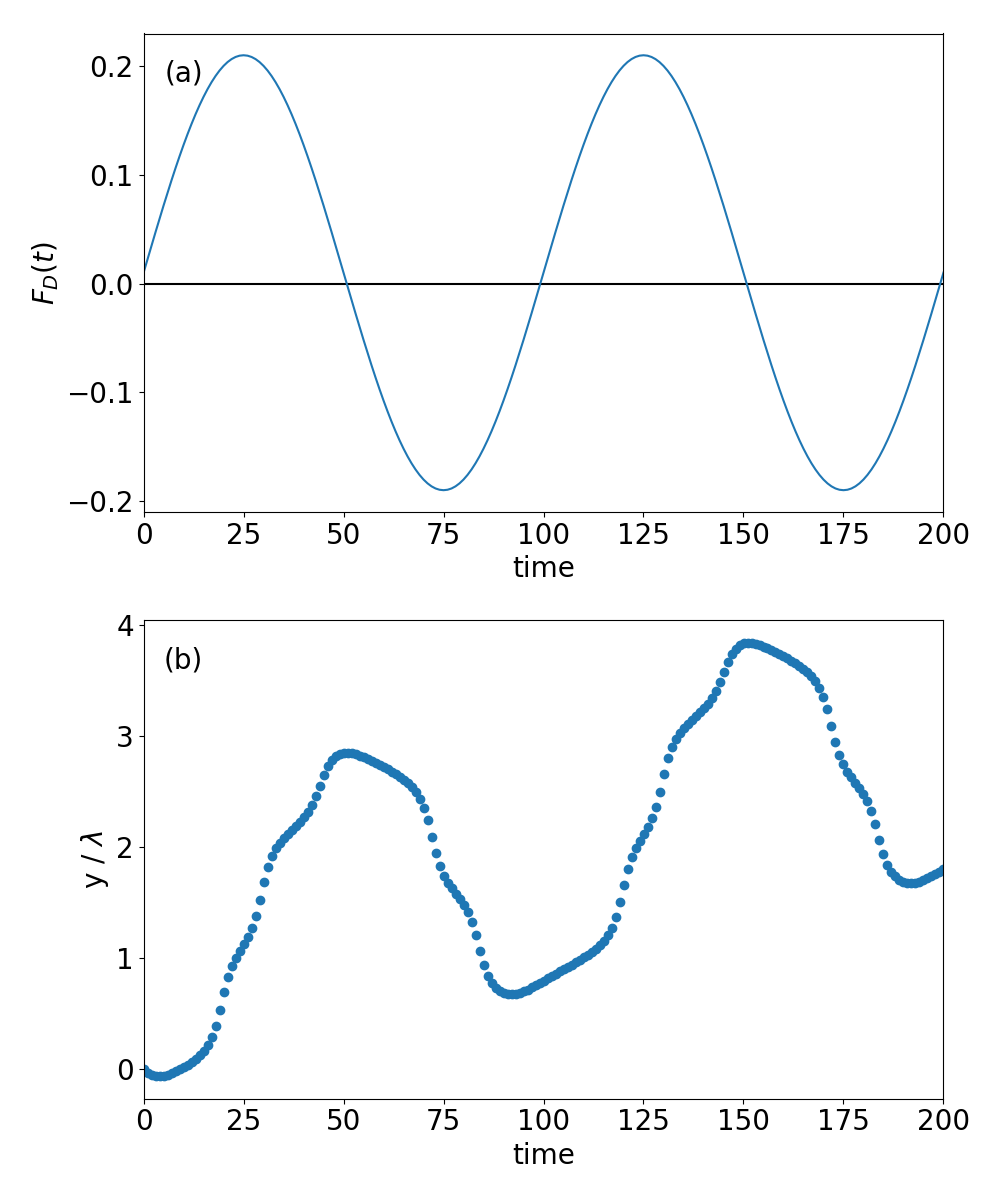
\includegraphics[width=\columnwidth]{position}
\caption{The position as a function of time of a single driven particle
  normalized by the period of the substrate $\lambda$.
  }
\label{fig:0}
\end{figure}
\end{center}

The hopping pattern of the driven particle is periodic,
and could be achieved over a range of $F_{DC}$.  %, as we will demonstrate in Fig.~\ref{fig:1}
We explore the ranges of periodic hopping patterns
by increasing $F_{DC}$ as a function of time,
as shown in 
%
Fig.~\ref{fig:1}.
%we show the result increasing the 
%force to the particle as a function of time.  
%increased DC
We apply an external applied force, 
with 
a constant $F_{AC}$ with frequency $\omega = 2\pi f$
then slowly increase $F_{DC}$
at a rate of $\Delta F_{DC} = 0.001$ every $\Delta t = 4000$ integer timesteps
or $40$ time units.
%this seems fast, but it is slow enough to estimate
%the velocity accurately.
%this is not be so for a multiple particle system!
By modifying $F_{DC}$ we 
achieve a variety of oscillation modes.
A mode is a periodic pattern of hops
with a constant average particle velocity, $\bar{v}_{y}$
over a range of driving forces $F_{DC}$.
We illustrate mode-locking in 
the velocity-force plot in Fig.~\ref{fig:1}(b).
Here $\bar{v}_{y}$ is increasing in non-uniform steps,
with a quantized height of
$\bar{v}_{y} = n \lambda f$,
where $n$ is an integer,
$\lambda = S_Y/N_p = 36.5/20 = 1.825$ is the spatial period, or wavelength
of the landscape,
and $f = 0.01$ cycles per time unit.

Our simulations reproduce results presented in 
Juniper {\it et al.} \cite{juniper2015}
which demonstrated
mode locking in
experiments of 
driven colloids on a
optical periodic landscape.

We illustrate the hopping pattern in Fig.~\ref{fig:1}(b)
and 
show the dynamics 
in supplementary materials \cite{supp1}.

\begin{center}
\begin{figure}[h!]
\centering
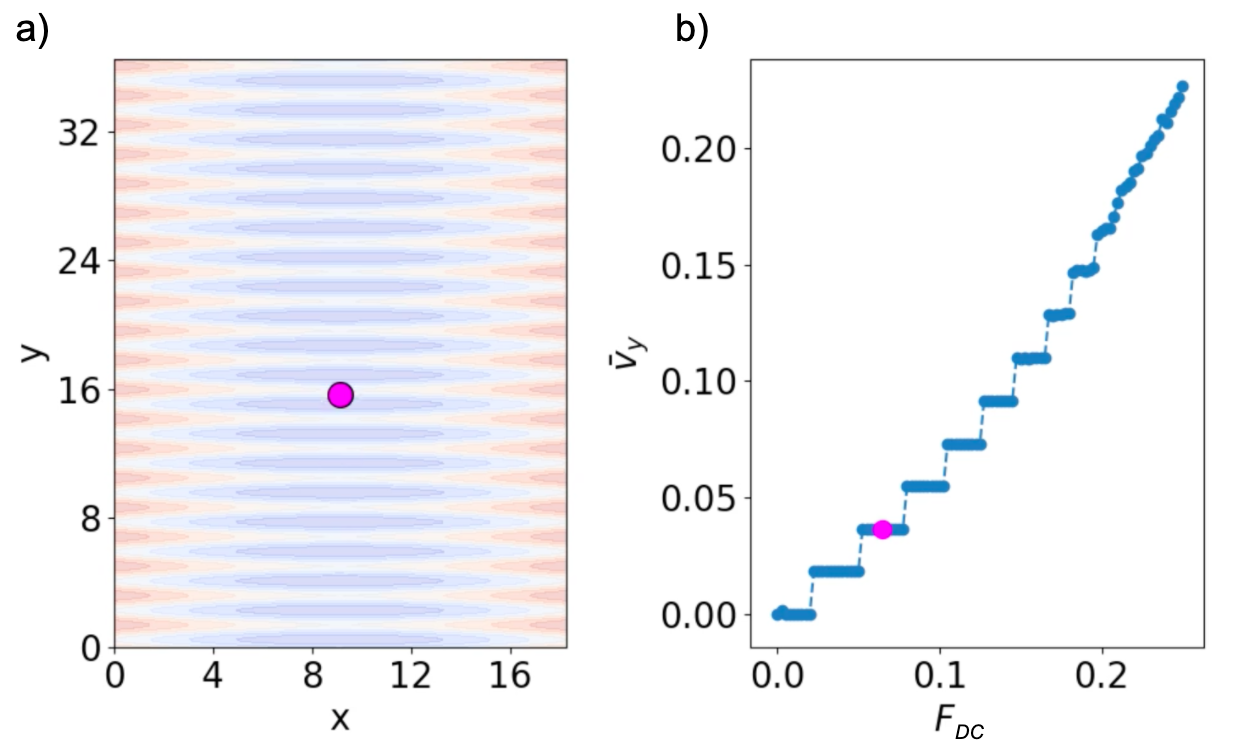
\includegraphics[scale=.25]{single}
\caption{\textbf{(a)} The particle is driven with a constant amplitude $F_{AC}$ and frequency $\omega$ through a periodic spatial potential landscape.  The landscape is represented with a colormap where blue are minima and red are maxima in the potential. \textbf{(b)} An average particle velocity in the y-direction $\bar{v}_{y}$ as a function of a constant driving force $F_{DC}$. In the animation available in Ref.~\cite{supp1} the magenta dot represents the average velocity of the particle $\bar{v}_{y}$ at which the particle in Fig. 1(a) is moving.}
\label{fig:1}
\end{figure}
\end{center}

\subsection{Synchronization in multi-particle systems}
\label{sec:sync}

We simulated a twenty particle system confined to a narrow channel, as shown in Fig. 2a).  We create the confining channel with a sinusoidal function
with a single period.
\begin{equation}
  \label{eq:channel}
  V_l(x) = V_{0x} \cos{(\pi x/L)}
\end{equation}
where the trough heights is larger  $V_{0x}$,
and the associated force
\begin{equation}
\vec{F}=-\nabla V(x) = -\frac{dV}{dx} \hat{x} = - \frac{V_{0x} \pi}{L} \sin{(\pi x/L)} \hat{x}
\end{equation}
restores particles to the center of a long narrow region of the simulation.
The landscape is illustrated in Fig.~\ref{fig:2}(a)
where red regions are high potential
and blue regions are low potential.

The initial configuration of the system is shown in 
Fig.~\ref{fig:2}(a).  
We annealed the system into a ground-state configuration
by raising the system to a high temperature $T$,
and slowly lowering the temperature in steps of $dT=-0.01$
until the particles form a buckled chain in the low region of the channel
due to the
competition between particle repulsion and channel confinement.
The interparticle forces between neighboring particles
cause the system to form a buckled chain. % when the system is annealed.
The molecular dynamics of simulated annealing
is described in Ref.~\ref{},
and presented simulations begin with particle configurations
that result from the annealing process,
as listed in Appendix [ref] and available in supplementary material.

When a single particle is driven, the neighboring particles act similarly to a periodic landscape to impede its motion. A driven particle can exhibit mode locking with a well-chosen AC drive and frequency. In the attached movie, Figure2.mp4, we show the complex dynamics of mode locking, where the driven particle leap-frogs past the other particles. 

\begin{center}
\begin{figure}[h!]
\centering
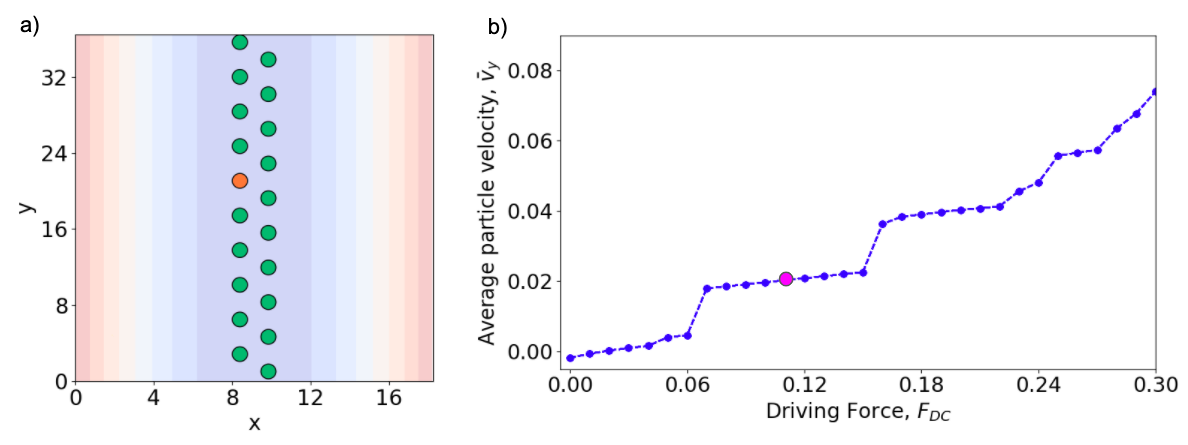
\includegraphics[scale=.40]{twenty}
\caption{\textbf{(a)} A single particle (colored orange - mark in some manner for non-color views) is driven with a constant amplitude $F_{AC}$ and frequency $\omega$ through 19 neighboring particles (colored green - mark differently) confined by a quasi one-dimensional channel. The landscape is colored as in Fig.~\ref{fig1}(a). \textbf{(b)} Average $\bar{v}_{y}$ versus $F_{DC}$, where $\bar{v}_{y}$ is the average particle velocity of the driven particle in the y-direction.}
\label{fig:2}
\end{figure}
\end{center}

\subsection{Kinked system}
\label{sec:kink}	% You can label sections for reference
We confine $N$ particles to $N-1$ troughs to create a
local high density region.
$F_{DC}/F_{AC} = 1$ [CHECK!]



\section{Quasiperiodic substrate}
\label{sec:quasiperiod}	% You can label sections for reference

\section{Chaotic dynamics}
\label{sec:chaos}	% You can label sections for reference

\section{Associated problems}
\label{sec:problems}	% You can label sections for reference


\section{Conclusion}
\label{sec:conclusion}	% You can label sections for reference

%%%%%%%%%%%%%%%%%%%%%%%%%%%%%%%%%%%%%%%%%%%%%%%%%%%%%%%%%%%%%%%%%%
\section{Supplementary Materials}

\subsection{Gridded Contour Plot of landscape}
%code is located in
%~/pymodules/animation_code/channel_colloid_movie_maker.py

\begin{verbatim}
##########################################################
#ADD CONTOUR PLOT
##########################################################
def add_contour(ax,L,N,corrugated = True):
    '''
    Hardwired to color in the quasi1D potential to contain 
    the particles in a trough.  
    Can also add the washboard/corrugated substrate.

    Required Arguments

    Optional Arguments:

    corrugated (default = True)  
    Adds the washboard in the y-direction.  
    Hardwired for a single parameter set.    
    '''

    a_p = L/N

    #assuming Tiare's trough system, so we won't want to cover the entire range
    X = np.arange(0, L/2.0, 0.1)
    Y = np.arange(0, L, 0.1)
    X, Y = np.meshgrid(X, Y)

    Z_mag = 2.0 # set by what "looks good"
    Z = Z_mag*np.sin(2*np.pi*X/L)
    if corrugated == True:
        Z += np.sin(2*np.pi*(Y+1.75)/a_p) 

    cmap=cm.coolwarm_r

    #alphs is the degree of transparency, again, set by what looks good.
    cset = ax.contourf(X, Y, Z, cmap=cmap,alpha=0.25)

    #ax1.set_xlim(15,20)
    #ax1.set_ylim(15,20)

    #ax1.set_xlabel(r"$X$")
    #ax1.set_ylabel(r"$y$",rotation='horizontal',ha='right')

    #ax1.set_xticks([])
    #ax1.set_yticks([])
    return
\end{verbatim}

\begin{acknowledgments}

  We acknowledge Harvey Gould and Jan Tobochnik,
  who invited us to write the article and
  supported its development.
  Charles and Cynthia Reichhardt advised 
  the project and provided the original molecular dynamics code
  written in the C programming language.
  We acknowledge funding from the M.J. Murdock Charitable Trust
  and the Pacific Research Institute for Science and Mathematics (PRISM).

\end{acknowledgments}


\begin{thebibliography}{99}
% The numeral (here 99) in curly braces is nominally the number of entries in
% the bibliography. It's supposed to affect the amount of space around the
% numerical labels, so only the number of digits should matter--and even that
  % seems to make no discernible difference.

  %useful quick ref
  %http://www.scholarpedia.org/article/Synchronization
  
  %intro to oscillators
\bibitem{Pikovsky2003} A. Pikovsky, M. Rosenblum, and J. Kurths, {\it Synchronization: A Universal Concept in Nonlinear Sciences} (Cambridge Univ. Press, Cambridge, 2003).
  
\bibitem{Bennett2002} M. Bennett, M.F. Schatz, H. Rockwood, and K. Wiesenfeld, Huygen's clocks, Proc. Roy. Soc. A {\bf 458}, 563 (2002).
  
\bibitem{Okamoto2016} K. Okamoto, A. Kijima, Y. Umeno, and H. Shima. Synchronization in flickering of three-coupled candle flames. Sci Rep {\bf 6}, 36145 (2016)

\bibitem{Jia2015}  J. Jia, Z. Song, W. Liu, J. Kurths, and Xiao, J. Experimental study of the triplet synchronization of coupled nonidentical mechanical metronomes. Sci. Rep. {\bf 5}, 17008 (2015).

  %biological examples
  
\bibitem{Portugal2014} S. Portugal, T. Hubel, J. Fritz, S. Heese, D. Trobe, B. Voelkl, S. Hailes, A. M. Wilson and J. R. Usherwood.  Upwash exploitation and downwash avoidance by flap phasing in ibis formation flight. Nature {\bf 505}, 399 (2014).

  \bibitem{Aihara2014} I. Aihara, T. Mizumoto, T. Otsuka, H. Awano, K. Nagira, H. G. Okuno and K. Aihara. Spatio-Temporal Dynamics in Collective Frog Choruses Examined by Mathematical Modeling and Field Observations. Sci Rep {\bf 4}, 3891 (2014). 

  \bibitem{Tranchant2016} P. Tranchant, D. T. Vuvan, and I. Peretz, Keeping the Beat: A Large Sample Study of Bouncing and Clapping to Music. PLoS ONE 11(7): e0160178. (2016).

  \bibitem{MartinHall1999} G. Martin Hall, Sonya Bahar, and Daniel J. Gauthier, Prevalence of Rate-Dependent Behaviors in Cardiac Muscle. Phys. Rev. Lett. {\bf 82}, 2995 (1999).

  \bibitem{Singer1999} W. Singer. Striving for coherence. Nature, {\bf 397} 391, 1999.

    %technological applications
    \bibitem{Dutta2019} Dutta, S., Parihar, A., Khanna, A. et al. Programmable coupled oscillators for synchronized locomotion. Nat Commun {\bf 10}, 3299 (2019).
    
    %condensed matter intro
    \bibitem{Bak1986} P. Bak. The Devil's Staircase. Physics Today {\bf 39}, 12, 38 (1986).

    \bibitem{Lissajous1857} J. A. Lissajous.  "Mémoire sur l'Etude optique des mouvements vibratoires,"  Annales de chimie et de physique, 3rd series, 51 (1857) 147-232

    \bibitem{Tong1997} E. Y. C. Tong, Lissajous figures The Physics Teacher {\bf 35}, 491 (1997).

    \bibitem{Josephson1962} B. D. Josephson, Phys. Letters {\bf 16}, 25 (1962). 
    \bibitem{Josephson1965} B. D. Josephson, Advan. Phys. {\bf 14}, 419 (1965).

    \bibitem{Stewart1968}  W. C. Stewart CURRENT‐VOLTAGE CHARACTERISTICS OF JOSEPHSON JUNCTIONS Appl. Phys. Lett. 12, 277 (1968).
      
    \bibitem{Shapiro1963} S. Shapiro, Josephson currents in superconducting tunneling: the effect of microwaves and other observations, Phys. Rev. Lett. 11, 80 (1963).

    \bibitem{Golubov2004} A. A. Golubov, M. Yu. Kupriyanov, and E. Il’ichev. The current-phase relation in Josephson junctions, Rev. Mod. Phys. {\bf 76}, 411 (2004).

      quote: Phase engineering techniques are used to control the dynamics of long-bosonic Josephson-junction arrays built by linearly coupling Bose-Einstein condensates.
    \bibitem{Zhang2020} Dengling Zhang, Haibo Qiu, and Antonio Muñoz Mateo, Unlocked-relative-phase states in arrays of Bose-Einstein condensates, Phys. Rev. A {\bf 101}, 063623 (2020).

      %reichhardt review
      %C. Reichhardt and C. J. Olson Reichhardt, “Depinning and nonequilibrium dynamic phases of particle assemblies driven over random and ordered substrates: a review,” Rep. Prog. Phys. 80, 026501 (2017).

    %  \bibitem{} Reichhardt, C., & Reichhardt, C. J. O. (2015). Shapiro steps for skyrmion motion on a washboard potential with longitudinal and transverse ac drives. Physical Review B - Condensed Matter and Materials Physics, 92(22). https://doi.org/10.1103/PhysRevB.92.224432
      
    \bibitem{juniper2015} M. P. N. Juniper, A. V. Straube, R. Besseling, D. G. A. L. Aarts, and R. P. A. Dullens, Microscopic dynamics of synchronization in driven colloids. Nat. Commun. 6, 7187 (2015).

    \bibitem{Bushev2013} P. Bushev, G. Hétet, L. Slodička, D. Rotter, M. A. Wilson, F. Schmidt-Kaler, J. Eschner, and R. Blatt, Shot-Noise-Limited Monitoring and Phase Locking of the Motion of a Single Trapped Ion, Phys. Rev. Lett. {\bf 110}, 133602 (2013).

\bibitem{supp1} See Figure1.mp4 in appropriate %\url{}

%\bibitem{latexsite} \LaTeX\ Project Web Site, \url{<http://www.latex-project.org/>}.

%\bibitem{wikibook} \textit{\LaTeX} (Wikibook), \url{<http://en.wikibooks.org/wiki/LaTeX/>}.

%\bibitem{latexbook}Helmut Kopka and Patrick W. Daly, \textit{A Guide to
%\LaTeX}, 4th edition (Addison-Wesley, Boston, 2004).

%\bibitem{revtex} REV\TeX\ 4 Home Page, \url{<https://authors.aps.org/revtex4/>}.

%\bibitem{cloudLaTeX} On the other hand, you can avoid the installation process
%entirely by using a cloud-based \LaTeX\ processor such as ShareLaTeX,
%\url{<https://www.sharelatex.com/>}, or write\LaTeX, \url{<https://www.writelatex.com/>}.

%\bibitem{nevermindlogic} In typography, aesthetics often takes precedence over logic.

%\bibitem{FontEncodingComment} Please don't try to handle foreign characters 
%and accents with the \texttt{inputenc} and \texttt{fontenc} packages, which 
%are incompatible with AJP's editing process.

%\bibitem{wikimathpage} See the Mathematics chapter of Ref.~\onlinecite{wikibook} for an excellent overview of math symbols and equations, with examples.

%\bibitem{labelnames} Thinking up a good label name takes a moment, but 
%it's worth the trouble; we strongly advise against using labels like 
%\texttt{eq2}, which become extremely confusing after you decide to add 
%another equation before Eq.~(\ref{deriv}).

%\bibitem{footnotes} You need to process a file twice to get the counters correct.

%\bibitem{mermin} N. David Mermin, ``What's wrong with these equations?,'' 
%Phys. Today \textbf{42} (10), 9--11 (1989).  
% Note that the issue number (10) in this citation is required, because
% each issue of Physics Today starts over with page 1.  Also note the use of
% an en-dash (--), not a hyphen (-), for the page range.

%\bibitem{editorsite} American Journal of Physics Editor's Web Site, 
%\url{<http://ajp.dickinson.edu>}.

%\bibitem{feynman} Richard P. Feynman, Robert B. Leighton, and Matthew Sands, 
%\textit{The Feynman Lectures on Physics, Vol.\ 1} (Addison-Wesley, 1964), p.~3-10.
% Note that this book is paginated by chapter; "3-10" is a single page reference
% that uses a hyphen, not a range of pages that would us an en-dash (--).

%\bibitem{noBIBTeX} Many \LaTeX\ users manage their bibliographic data with 
%a tool called BIB\TeX.  Unfortunately, AJP cannot accept BIB\TeX\ files; all 
%bibliographic references must be incorporated into the manuscript file
%as shown here, at least when you send an editable file for production.

%\bibitem{dyson} Freeman J. Dyson, ``Feynman's proof of the Maxwell equations,''
%Am. J. Phys. \textbf{58} (3), 209--211.  
% The issue number (3) in this citation is optional, because AJP's pagination 
% is by volume.

%\bibitem{examplevolume} M. R. Flannery, ``Elastic scattering,'' in 
%\textit{Atomic, Molecular, and Optical Physics Handbook}, edited by
%G. W. F. Drake (AIP Press, New York, 1996), p.~520.

%\bibitem{AIPstylemanual} \textit{AIP Style Manual}, 4th edition (American 
%Institute of Physics, New York, 1990). Available online at 
%\url{<http://www.aip.org/pubservs/style/4thed/toc.html>}. Although parts of 
%it have been made out of date by advancing technology, most of this manual 
%is still as useful as ever. Just be sure to follow AJP's specific rules
%whenever they conflict with those in the manual.

\end{thebibliography}

% If your manuscript is conditionally accepted, the editors will ask you to
% submit your editable LaTeX source file.  Before doing so, you should move
% all tables and figure captions to the end, as shown below.  Tables come 
% first, followed by figure captions (with figure inclusions commented-out).
% Figures should be submitted as separate files, collected with the
% LaTeX file into a single .zip archive.

%\newpage   % Start a new page for tables

%\begin{table}[h!]
%\centering
%\caption{Elementary bosons}
%\begin{ruledtabular}
%\begin{tabular}{l c c c c p{5cm}}
%Name & Symbol & Mass (GeV/$c^2$) & Spin & Discovered & Interacts with \\
%\hline
%Photon & $\gamma$ & \ \ 0 & 1 & 1905 & Electrically charged particles \\
%Gluons & $g$ & \ \ 0 & 1 & 1978 & Strongly interacting particles (quarks and gluons) \\
%Weak charged bosons & $W^\pm$ & \ 82 & 1 & 1983 & Quarks, leptons, $W^\pm$, $Z^0$, $\gamma$ \\
%Weak neutral boson & $Z^0$ & \ 91 & 1 & 1983 & Quarks, leptons, $W^\pm$, $Z^0$ \\
%Higgs boson & $H$ & 126 & 0 & 2012 & Massive particles (according to theory) \\
%\end{tabular}
%\end{ruledtabular}
%\label{bosons}
%\end{table}

%\newpage   % Start a new page for figure captions

%\section*{Figure captions}

%\begin{figure}[h!]
%\centering
%\includegraphics{GasBulbData.eps}   % This line stays commented-out
%\caption{Pressure as a function of temperature for a fixed volume of air.  
%The three data sets are for three different amounts of air in the container. 
%For an ideal gas, the pressure would go to zero at $-273^\circ$C.  (Notice
%that this is a vector graphic, so it can be viewed at any scale without
%seeing pixels.)}

%\label{gasbulbdata}
%\end{figure}

%\begin{figure}[h!]
%\centering
%\includegraphics[width=5in]{ThreeSunsets.jpg}   % This line stays commented-out
%\caption{Three overlaid sequences of photos of the setting sun, taken
%near the December solstice (left), September equinox (center), and
%June solstice (right), all from the same location at 41$^\circ$ north
%latitude. The time interval between images in each sequence is approximately
%four minutes.}
%\label{sunsets}
%\end{figure}
      
\end{document}

\begin{equation}
\vec{F}_{D}(t) = [F_{DC} + F_{AC} \sin(2 \pi f t)] \hat{y} 
\end{equation}

\begin{equation}
F_{DC} = 0.01
\end{equation}

\begin{equation}
F_{AC} = 0.2 
\end{equation}

\begin{equation}
f = 0.01 
\end{equation}

\begin{equation}
\bar{v}_y = n \lambda f
\end{equation}

\begin{equation}
\bar{v}_y = \lambda f
\end{equation}

\begin{equation}
\lambda = S_Y / 20
\end{equation}

\begin{equation}
F_{p} = 0.1
\end{equation}

%%%%%%%%%%%%%%%%%%%%%%%%%%%%%%%%%%%%%%%%%%%%%%%%%%%%%%%%%%%%%%%%%%
\section{Supplementary Materials}

\subsection{Gridded Contour Plot of landscape}
%code is located in
%~/pymodules/animation_code/channel_colloid_movie_maker.py

\begin{verbatim}
##########################################################
#ADD CONTOUR PLOT
##########################################################
def add_contour(ax,L,N,corrugated = True):
    '''
    Hardwired to color in the quasi1D potential to contain 
    the particles in a trough.  
    Can also add the washboard/corrugated substrate.

    Required Arguments

    Optional Arguments:

    corrugated (default = True)  
    Adds the washboard in the y-direction.  
    Hardwired for a single parameter set.    
    '''

    a_p = L/N

    #assuming Tiare's trough system, so we won't want to cover the entire range
    X = np.arange(0, L/2.0, 0.1)
    Y = np.arange(0, L, 0.1)
    X, Y = np.meshgrid(X, Y)

    Z_mag = 2.0 # set by what "looks good"
    Z = Z_mag*np.sin(2*np.pi*X/L)
    if corrugated == True:
        Z += np.sin(2*np.pi*(Y+1.75)/a_p) 

    cmap=cm.coolwarm_r

    #alphs is the degree of transparency, again, set by what looks good.
    cset = ax.contourf(X, Y, Z, cmap=cmap,alpha=0.25)

    #ax1.set_xlim(15,20)
    #ax1.set_ylim(15,20)

    #ax1.set_xlabel(r"$X$")
    #ax1.set_ylabel(r"$y$",rotation='horizontal',ha='right')

    #ax1.set_xticks([])
    #ax1.set_yticks([])
    return
\end{verbatim}
